\documentclass[10pt,spanish,a4paper,openany,notitlepage]{article}
%-------------------------------------Paquetes-----------------------------------------------------------------------
\usepackage[spanish,es-tabla]{babel}  	% Traduce los textos a castellano
\usepackage[utf8]{inputenc}	% Permite escribir directamente áéíóúñ
\usepackage{t1enc}            	% Agrega caracteres extendidos al font
\usepackage{amsmath} 		%Permite imprimir mas opciones matemáticas
\usepackage{graphicx}		%Permite agregar imagenes al informe
\usepackage{float} 		%Permite utilizar H para colocar las imagenes en un lugar especifico 
\usepackage{units}
\usepackage{circuitikz}
\usepackage{caption}
\usepackage{subcaption}
\usepackage{sidecap}
\usepackage{mathtools}
\usepackage{multirow} % Paquete para dividir las tablas en subtablas
\usepackage{booktabs} %estos 2 sirven para achicar la tabla
\usepackage{tabulary}
\usepackage{fancyhdr} % encabezado
\usepackage{textcomp} % para usar ° con el comando \textdegree
\usepackage{anysize}		%Permite modificar los margenes del documento
\usepackage{abstract} % paquete para el resumen del articulo
\usepackage{amssymb}





% todo lo que sigue es para poner links que se les pueda hacer click
\usepackage{xcolor}
\usepackage[normalem]{ulem}
\usepackage{hyperref}
\hypersetup{colorlinks,urlcolor=blue}

\makeatletter
\DeclareUrlCommand\ULurl@@{%
  \def\UrlFont{\ttfamily\color{blue}}%
  \def\UrlLeft{\uline\bgroup}%
  \def\UrlRight{\egroup}}
\def\ULurl@#1{\hyper@linkurl{\ULurl@@{#1}}{#1}}
\DeclareRobustCommand*\ULurl{\hyper@normalise\ULurl@}
\makeatother

%---------------------------------------Configuraciones de pagina----------------------------------------------
\marginsize{2.5cm}{2.5cm}{1cm}{1cm}

\pagestyle{fancy}
\fancyhf{}
\lhead{
66.09 - \textsc{Laboratorio de Microcomputadoras}\\ 
1\textsuperscript{er} Cuatrimestre de 2015
}
\rhead{
\includegraphics[width=3cm]{imagenes/FIUBA_ALTA.jpg}}
\rfoot{Página \thepage}

%---------------------------------------Definiciones propias---------------------------------------------------------
\newcommand{\oiint}{\displaystyle\bigcirc\!\!\!\!\!\!\!\!\int\!\!\!\!\!\int} %Integral doble cerrada

\DeclarePairedDelimiter\abs{\lvert}{\rvert}%
\DeclarePairedDelimiter\norm{\lVert}{\rVert}%
% Swap the definition of \abs* and \norm*, so that \abs
% and \norm resizes the size of the brackets, and the 
% starred version does not.
\makeatletter
\let\oldabs\abs
\def\abs{\@ifstar{\oldabs}{\oldabs*}}
%
\let\oldnorm\norm
\def\norm{\@ifstar{\oldnorm}{\oldnorm*}}
\makeatother
%--------------------------------------------------------------------------------------------------------------------------------


\makeatletter
\let\ps@plain\ps@fancy 
\makeatother

% lo siguiente es para borrar el titulo del resumen y que no ocupe espacio:
 \AtBeginDocument{%
 \renewcommand{\abstractname}{}%
 }
\renewcommand{\absnamepos}{empty} % originally center
 

\begin{document}
\title{\textbf{Proyecto: Dispositivo autorregulador de la percepción térmica corporal}}
\author{
  Martinez, Gaston - 91383\\
  \texttt{gaston.martinez.90@gmail.com}  
  \and
   Vázquez, Matías - 91523\\
  \texttt{mfvazquez@gmail.com}
}
\date{\today}
\maketitle

\begin{abstract} %Resumen
\emph{Se diseñará e implementará una pulsera térmica que regulará la
temperatura corporal. Se utilizará un módulo termoeléctrico para enviar
variaciones de calor o frío a la muñeca del usuario para modificar
la percepción térmica del cuerpo.}
\end{abstract}

\section{Introducción}

Su función es generar pulsos de frío o calor, de manera de generar una sensación de 
confort para una persona en condiciones donde la temperatura es muy alta 
o muy baja respectivamente.
Está basado en el proyecto \emph{Wristify} \cite{embrlabs} ganador del concurso de intel 
\emph{Make It Wearable} \cite{Make It Wearable}.

\section{Especificaciones}

El dispositivo utilizará una celda Peltier para enviar pulsos de calor
o frío. De forma que se logre una diferencia de temperatura de $0,4\, \unit{^oC/seg.}$
durante 5 segundos y durante los siguientes 10 segundos entrará
en estado de espera, para luego volver a iniciar el ciclo. 

Deberá contar con un sensor de temperatura para medir la temperatura ambiente
y analizar si deberá enviar o recibir calor.

Finalmente deberá controlar que se cumpla el ciclo utilizando una termocupla
para medir la temperatura corporal cercana a la placa de peltier.

\subsection{Componentes}

Deberá contar con los siguientes componentes.

\begin{itemize}
\item{Placa de peltier:} Generará los pulsos térmicos en la muñeca del usuario.
\item{Termómetro:} Medirá la temperatura ambiente y en base a ella decidirá 
si se debe aumentar o reducir la temperatura en la termocupla.
\item{Termocupla:} Contará con una doble finalidad. Por un lado permitirá 
medir el cambio de temperatura de la placa; y por el otro permitirá medir 
la temperatura actual del cuerpo al momento de colocarse la pulsera.
\item{Salida de puerto serie:} Servirá para poder monitorear en una 
computadora la temperatura de la placa.
\item{Fuente:} Se encargará de suministrar la corriente necesaria a la 
placa de peltier y proporcionará alimentación a todos los dispositivos utilizados.
\item{Pulsador:} Para poder invertir el estado de trabajo, de frío a calor 
y viceversa.
\item{Disipador:} Se encargará de disipar el calor del lado opuesto al de 
la muñeca de la placa de peltier.
\item{Controlador:} Se utilizara un microcontrolador AVR. Recibirá la temperatura ambiente del termómetro
para decidir que régimen de trabajo establecer, y con la temperatura suministrada por la termocupla
decidirá cuanta corriente suministrarle a la celda Peltier mediante un circuito regulador de corriente.
También estará conectado a un pulsador para invertir el régimen de trabajo.
\end{itemize}

\subsection{Diagrama de Flujo}

\begin{figure}[H] %[h] para here [b] para bottom [t] para top [H]+float para aqui si o si
\begin{center}
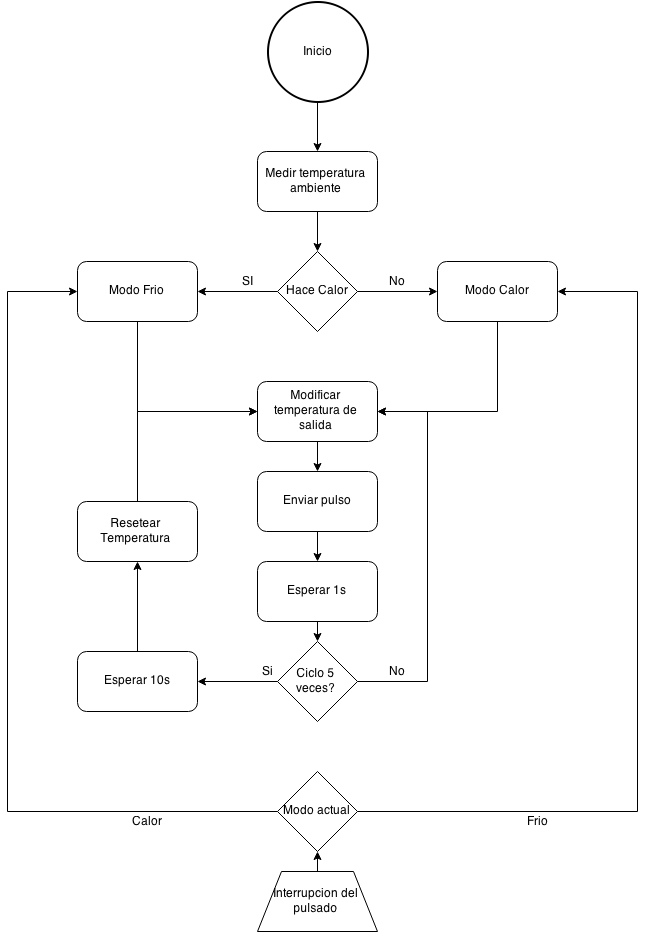
\includegraphics[scale=0.6]{./imagenes/diagrama_de_flujo.png}
\caption{Diagrama de flujo del proceso}
 \label{fig:diag_flujo}
\end{center}
\end{figure}

\subsection{Diagrama de Bloques}

\begin{figure}[H] %[h] para here [b] para bottom [t] para top [H]+float para aqui si o si
\begin{center}
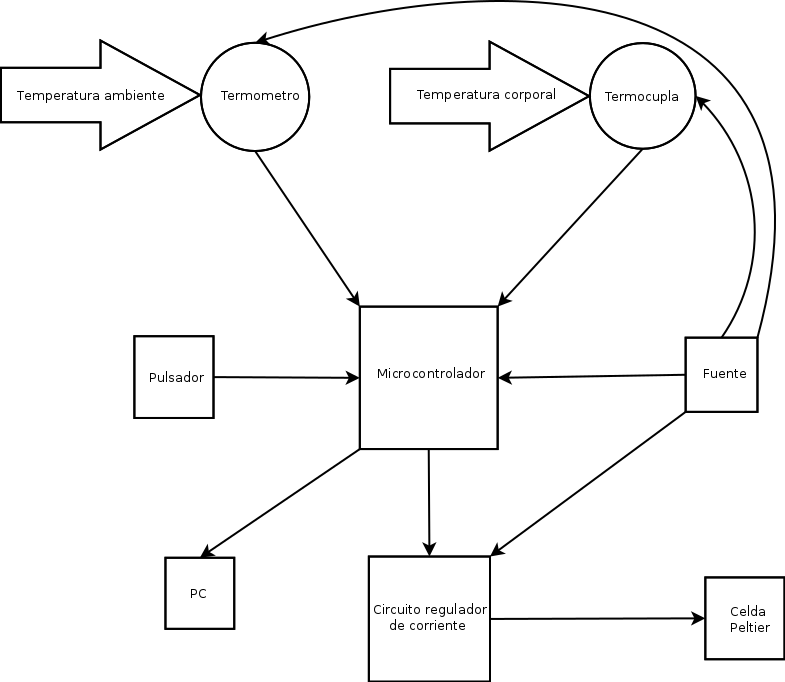
\includegraphics[scale=0.5]{./imagenes/diagrama_de_bloques.png}
\caption{Diagrama de bloques}
 \label{fig:diag_bloques}
\end{center}
\end{figure}


\section{Diseño}

\subsection{Circuito regulador de corriente}

Para la construcción del circuito regulador de corriente se utilizará
un regulador de tensión {\bf LM317}. Partiendo del circuito mostrado
en la figura número \ref{circuito:reg_corriente}. Se obtendrá el
valor mínimo de $R_1$ para obtener la corriente máxima de salida $I_{out}$
mediante la ecuación número \ref{eq:iout}.

\begin{figure}[H]
\centering
\begin{circuitikz}[american]\shorthandoff{>}
\draw
(0,0) to [short] (9.5,0)
to [short] (2.5,1)
to [short] (0,1)
to [short] (0,0)
(0,0.10) to [open,l=\bf{LM317}] (2.5,0.10)
 
(2.5,0.5) to [R, l=$R_1$] (5, 0.5)
to [short, -o , i=$I_{out}$] (6.5, 0.5)

(1.25, 0) to [short] (1.25, -1)
to [short] (5, -1)
to [short, -*] (5, 0.5)

(-1, 0.5) to [short, o-, l= $V_{in}$] (0, 0.5)

;\end{circuitikz}
\caption{Circuito regulador de corriente}
\label{circuito:reg_corriente}
\end{figure}

\begin{equation}
I_{out} = \frac{1.25\, \unit{V}}{R_1}
\label{eq:iout}
\end{equation}
 
La corriente máxima de salida será necesaria para alcanzar una diferencia 
de temperatura de $2\, \unit{^oC}$ entre una de las caras de la celda Peltier 
y la temperatura ambiente. Que se deberá obtener experimentalmente con
la celda Peltier utilizada.

\section{Especificaciones del microcontrolador}

\subsection{Microcontrolador}
Para este proyecto se utilizo un microcontrolador \texttt{Atmega8L}. El datasheet del mismo se puede obtener en la pagina de Atmel\cite{datasheet}
\subsection{Configuraciones}
\subsubsection{Clock}
El clock del microcontrolador fue establecido en 8MHz. 
\begin{center}
\begin{tabular}{|c|c|c|c|c|c|c|c|}\hline
7&6&5&4&3&2&1&0\\\hline
a&a&a&a&a&a&a&a\\\hline
0&0&0&0&0&0&0&0\\\hline
\end{tabular}
\end{center}
\subsubsection{PWM}
El PWM 
\subsection{}

\newpage
\begin{thebibliography}{9}

\bibitem{embrlabs}
  \ULurl{http://www.embrlabs.com/}

\bibitem{Make It Wearable}
  \ULurl{https://youtu.be/sDZHITVfYrI}
  
\bibitem{video MIT}
  \ULurl{https://youtu.be/kvUMCip-r4A}

\bibitem{datasheet}
  \ULurl{http://www.atmel.com/images/atmel-2486-8-bit-avr-microcontroller-atmega8_l_datasheet.pdf}

\end{thebibliography}

\end{document}
